\graphicspath{{content/chapters/2_background/figures/}}
\chapter{Background}
\label{chp:background}

In this chapter, background information on established classical noise reduction methods is provided. It explores Spectral Subtraction, Wiener Filtering, and MMSE-LSA estimation, which does not require reference signals.  The chapter introduces the key evaluation metrics used to assess speech enhancement performance. Additionally, a brief section outlines the progression of the project and relevant foundational knowledge.

\section{Spectral Subtraction}
\label{sec:spectral_subtraction}

\gls{ss} is one of the most widely used techniques for single-channel speech enhancement. The core idea is to estimate the noise spectrum from a noisy speech signal and subtract it from the observed spectrum to obtain a cleaner signal \cite{loizou2013speech}. It assumes that noise remains relatively stationary over short time frames, while speech is a dynamic, non-stationary signal.

The analog speech signal \(x(t)\) must be digitised into \gls{x}, a discrete-time signal. This digitisation must satisfy the Nyquist criterion, sampling at a rate at least twice the maximum frequency for accurate representation. However, sampling introduces limitations, such as quantisation noise and aliasing. If the sampling rate is too low, high-frequency components may fold into lower frequencies, misrepresenting the signal content \cite{loizou2013speech}.

\begin{figure}[h]
    \centering
    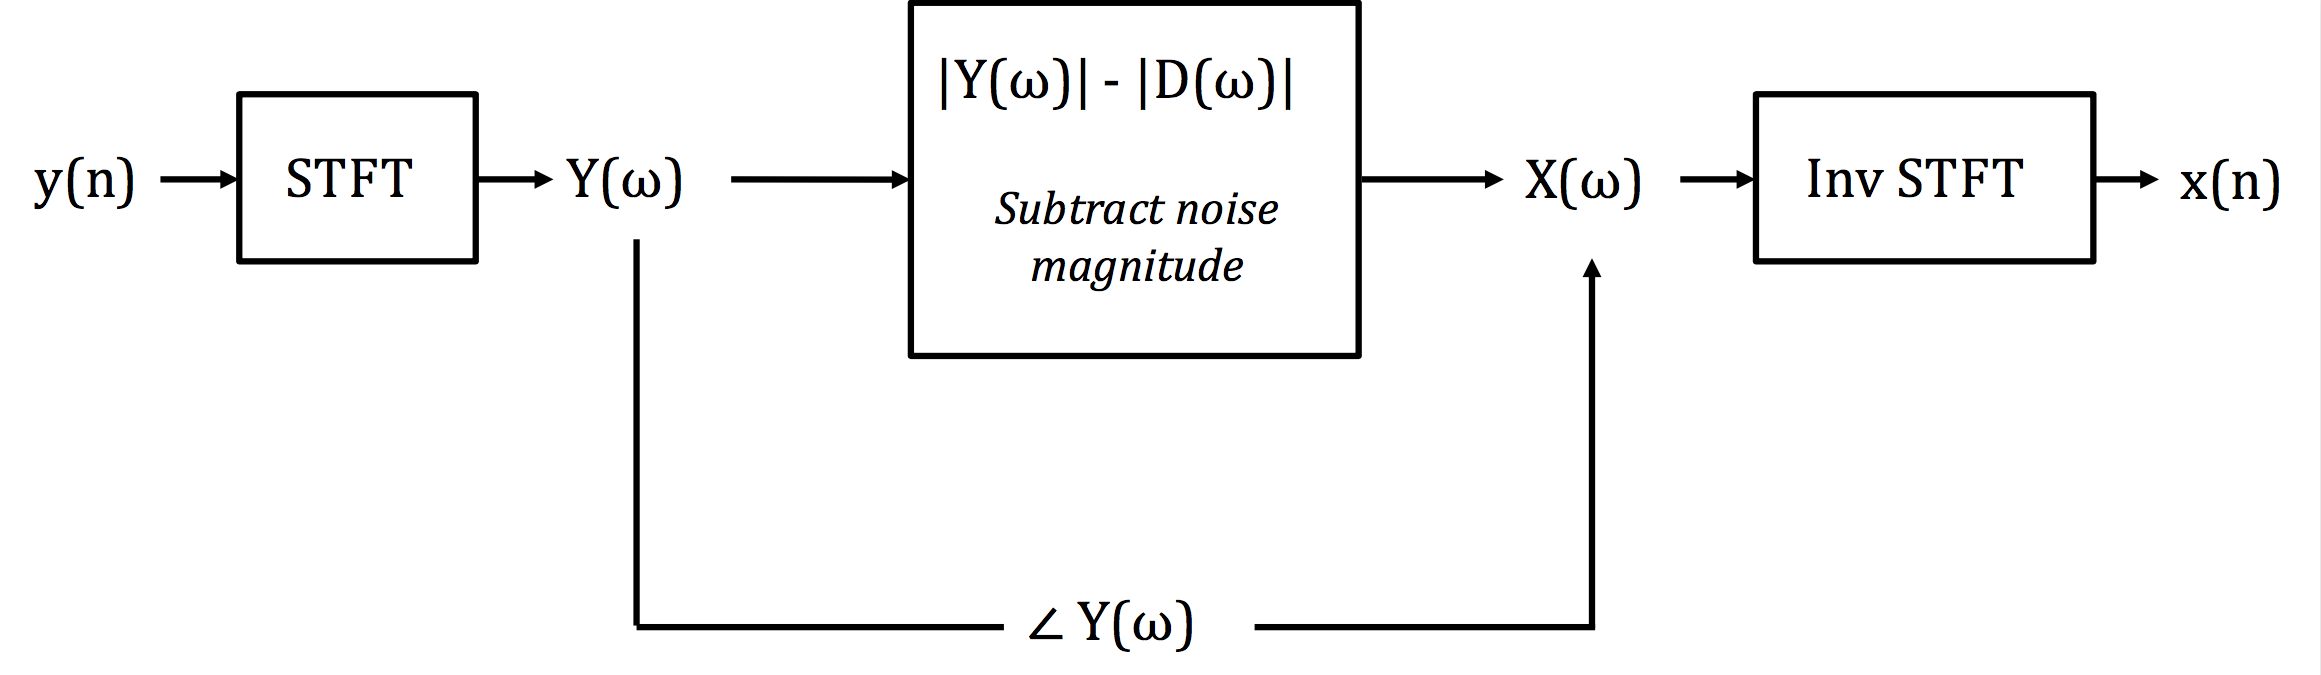
\includegraphics[width=\textwidth,keepaspectratio]{specsub.png}
    \caption{\label{fig:SSBlock} Block diagram of the Spectral Subtraction method \cite{dubey2016evaluation}.}
\end{figure}

Before applying \gls{ss}, the signal is pre-processed into a suitable format using the \gls{stft}. The \gls{stft} segments the time-domain signal into overlapping frames using a windowing function and then converts each segment into the frequency domain. Windowing reduces spectral leakage and preserves continuity in the frequency domain. The magnitude spectrum of the noisy signal is obtained by taking the absolute value of the \gls{stft} \cite{dubey2016evaluation}. The noise spectrum is estimated by averaging the spectral magnitudes of non-speech segments over time. Once this estimate is obtained, it is subtracted from the noisy spectrum to yield an estimate of the clean speech. The final step applies the \gls{istft} to reconstruct the enhanced signal in the time domain by summing the overlapping frames.

This process can be mathematically described as:

\begin{equation}
    \gls{Xomega} = \gls{Yomega} - \gls{Domega}
\end{equation}

\gls{ss} is widely adopted due to its simplicity and low computational cost. It requires only a single input channel and is straightforward to implement. However, it assumes stationary noise, a condition often unmet in practice. It may also introduce musical noise, a type of distortion perceived as tonal artifacts. Excessive subtraction may distort speech, while insufficient subtraction can leave residual noise.

Despite these challenges, \gls{ss} remains a valuable baseline for evaluating more advanced noise suppression techniques. Methods such as Wiener filtering and deep learning-based approaches have been developed to overcome these shortcomings through more adaptive or data-driven mechanisms \cite{loizou2013speech}.


\section{Wiener Filtering}
\label{sec:wiener_filtering}

\gls{wf} is a statistically grounded method for speech enhancement that aims to minimise \gls{mse} between the estimated clean signal and the true clean signal \cite{loizou2013speech}. Originally developed for linear time-invariant systems, the Wiener filter assumes that both the signal and noise are stationary stochastic processes and seeks the optimal linear estimate of the clean speech given the noisy observation \cite{dubey2016evaluation}.

Though usable in time or frequency domains, the frequency version is preferred for efficiency and \gls{stft} compatibility. The key idea is that if the power spectral densities (PSDs) of the clean speech \gls{Ps} and the noise \gls{Pn} are known or can be estimated, the optimal filter \gls{Homega} is derived as:

\begin{equation}
    \gls{Homega} = \frac{\gls{Ps}}{\gls{Ps} + \gls{Pn}}
\end{equation}

This filter acts as a frequency-dependent gain function. Frequencies where the clean speech dominates (\(P_S \gg P_N\)) are preserved, while noise dominant frequencies (\(P_N \gg P_S\)) are attenuated. The enhanced speech spectrum is obtained by multiplying the noisy spectrum \(Y(\omega)\) with the Wiener gain:

\begin{equation}
    \gls{xhatomega} = \gls{Homega}Y(\omega)
\end{equation}

The enhanced signal is then reconstructed using the \gls{istft}.

\begin{figure}[h]
    \centering
    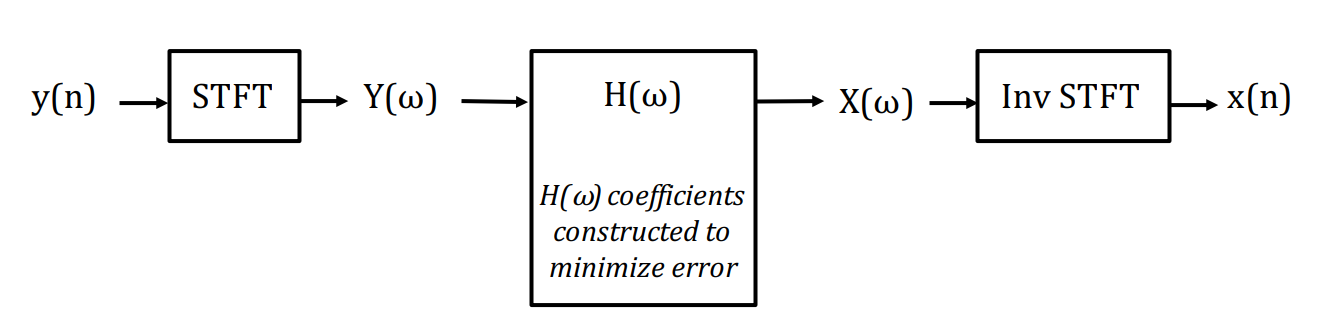
\includegraphics[width=0.95\textwidth,keepaspectratio]{wiener_block.png}
    \caption{\label{fig:WienerBlock} Block diagram of the Weiner Filtering process \cite{dubey2016evaluation}.}
\end{figure}

\gls{wf} is a statistically optimal method that minimizes the mean square error (MMSE) between the estimated and clean speech signals. It performs well when noise characteristics can be reliably estimated, such as during silent speech segments, and is effective at preserving the spectral shape of speech components. However, the method assumes stationary, zero-mean noise uncorrelated with the speech signal. These assumptions often fail in real-world, dynamic environments. This can lead to inaccurate power spectral density (PSD) estimates, resulting in performance degradation or over-smoothing that reduces intelligibility.

Despite these limitations, \gls{wf} remains a foundational approach in speech enhancement and is frequently integrated into more advanced or hybrid denoising pipelines \cite{dubey2016evaluation, loizou2013speech}.


\section{Minimum Mean Square Error Log-Spectral Amplitude Estimation}
\label{sec:mmse_lsa}

The \gls{mmse-lsa} estimator is a statistically grounded single-channel speech enhancement technique first proposed by Ephraim and Malah in 1984~\cite{ephraim1984speech}. Unlike \gls{ss} and \gls{wf}, which operate on magnitude or power spectra. \gls{mmse-lsa} aims to minimise the mean-square error between the logarithm of the spectral amplitudes of the clean and enhanced speech signals.

The algorithm operates in the time/frequency domain, assuming additive noise and using the \gls{stft} to decompose the noisy signal. It relies on estimates of the a priori and a posteriori signal-to-noise ratios (SNRs) to construct a gain function that enhances speech-dominant regions while suppressing noise. The enhanced spectral amplitude \( \hat{X}^{\text{LSA}}(\omega) \) is computed as:

\begin{equation}
    \hat{X}^{\text{LSA}}(\omega) =\exp (\mathrm{E} \log(\gls{Xomega} \gls{Yomega}))
\end{equation}
where \gls{Yomega} is the noisy observation and the expectation is taken over the distribution of the clean signal conditioned on the observed noisy spectrum.

A block diagram of the \gls{mmse-lsa} estimation process is made and shown in Figure~\ref{fig:mmse_lsa_block}. It begins with an \gls{stft} of the input signal, followed by separation into magnitude and phase. The magnitude spectrum is used to estimate the noise power spectral density (PSD), from which the a priori and a posteriori SNRs are derived. These estimates are then passed into the \gls{mmse-lsa} gain function, which produces a gain mask applied to the magnitude spectrum. The enhanced signal is reconstructed by combining the modified magnitude with the original phase, followed by the inverse \gls{stft}.

\begin{figure}[H]
    \centering
    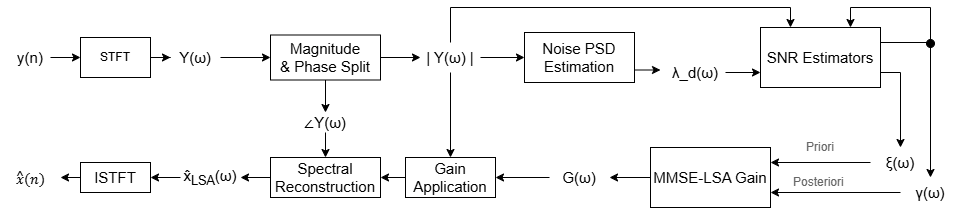
\includegraphics[width=\textwidth]{mmse-lsa.png}
    \caption{\label{fig:mmse_lsa_block} Block diagram of the MMSE-LSA method}
\end{figure}

The \gls{mmse-lsa} estimator incorporates a parametric model of the speech and noise distributions and uses recursive averaging to smooth \gls{snr} estimates across time frames. This results in a more adaptive and perceptually aligned gain function than traditional methods. This log-domain formulation better aligns with human auditory perception.

Despite its original formulation in the 1980s, \gls{mmse-lsa} continues to be a highly relevant technique. Numerous enhancements and application-specific variants have been developed in the 2010s and 2020s, including integrations with wavelet transforms~\cite{wei2016mmse} and hybrid neural-\gls{dsp} pipelines for hearing aids~\cite{sugahara2024hybrid}. This enduring relevance highlights \gls{mmse-lsa}'s foundational robustness and its suitability for modern speech enhancement systems.

\section{Evaluation Metrics}
\label{sec:evaluation_metrics}

To evaluate the performance of noise reduction algorithms, several objective metrics are commonly used. These metrics provide quantitative measures of the quality and intelligibility of enhanced speech signals when compared to their clean references. The following subsections describe the most widely adopted metrics in speech enhancement research, all of which are utilised in this project.

\subsection{Signal-to-Noise Ratio}
\label{subsec:snr}

The \gls{snr} is a fundamental metric that quantifies the relative strength of the desired speech signal compared to the background noise. A higher \gls{snr} indicates better separation between speech and noise components, which typically translates to improved intelligibility and perceived quality.

\gls{snr} is defined as:

\begin{equation}
    \text{SNR} = 10 \log_{10} \left( \frac{P_s}{P_n} \right)
\end{equation}

where \( P_s \) is the power of the clean speech signal and \( P_n \) is the power of the noise (or error) component. In practice, \gls{snr} can be computed in both time and frequency domains and is commonly used as a baseline performance indicator for denoising systems.

\subsection{Mean Squared Error}
\label{subsec:mse}

The \gls{mse} measures the average squared difference between the enhanced and reference clean signals. It reflects the overall fidelity of the enhancement process but does not necessarily correlate with perceptual quality.

\gls{mse} is given by:

\begin{equation}
    \text{MSE} = \frac{1}{\gls{N}} \sum_{n=1}^{\gls{N}} (\gls{x} - \gls{xhat})^2
\end{equation}

where \gls{N} is the number of signal samples, \gls{x} is the clean signal, and \gls{xhat} is the enhanced signal. Lower \gls{mse} values indicate better approximation of the clean signal.

\subsection{Perceptual Evaluation of Speech Quality}
\label{subsec:pesq}

The \gls{pesq} is an objective metric designed to estimate the perceptual quality of speech, taking into account human auditory perception. Standardised \cite{itutp862}, \gls{pesq} is widely used in speech enhancement and telecommunication systems.

\gls{pesq} simulates the auditory perception process and compares the clean and enhanced signals using psychoacoustic models. The \gls{pesq} score ranges from -0.5 to 4.5, with higher scores indicating better perceptual quality. A score above 3.0 is generally considered acceptable for most applications.

\subsection{Short-Time Objective Intelligibility}
\label{subsec:stoi}

The \gls{stoi} metric is designed to assess the intelligibility of speech, especially in noisy or distorted conditions. Proposed by Taal et al.~\cite{taal2011stoi}, it works by comparing the short-time spectral envelopes of clean and enhanced speech segments.

The \gls{stoi} score lies between 0 and 1, where higher values indicate better intelligibility. Scores above 0.5 typically suggest acceptable levels of speech understanding. \gls{stoi} is particularly useful when intelligibility, rather than perceptual quality alone, is of primary concern.

\subsection{Log Spectral Distance}
\label{subsec:lsd}

The \gls{lsd} metric quantifies the spectral distortion introduced by a denoising algorithm. It measures the average distance between the logarithmic power spectra of the clean and enhanced signals across time and frequency. This metric has been widely used in speech enhancement tasks, as seen in works such as~\cite{kubichek1993lsd}.

\gls{lsd} is defined as:

\begin{equation}
    \text{LSD} = \frac{1}{F} \sum_{f=1}^{F} \sqrt{ \frac{1}{T} \sum_{t=1}^{T} \left( \log \gls{Sft} - \log \gls{Shft} \right)^2 }
\end{equation}

where \gls{Sft} and \gls{Shft} are the clean and enhanced magnitude spectra at frequency bin \( f \) and time frame \( t \), respectively. Lower \gls{lsd} values indicate better preservation of spectral characteristics and less distortion.

\vspace{2em}
Individually, these metrics fail to provide a complete and meaningful evaluation of the performance of noise reduction algorithms. For example, \gls{snr} and \gls{mse} are sensitive to the absolute power levels of the signals, while \gls{pesq} and \gls{stoi} focus on perceptual aspects. Thus, multiple metrics are needed for a well rounded assessment.


\section{Project Progression}
\label{sec:project_progression}

The initial objective of this project was to enhance speech signals corrupted by noise using traditional \gls{dsp} techniques. The original scope involved implementing classical noise reduction methods, such as \gls{ss} and \gls{wf}, with the intention of deploying them on an MSP432 microcontroller. These techniques were selected due to their low computational complexity and suitability for resource-constrained embedded systems.

However, early prototyping in Python revealed inherent limitations of classical \gls{dsp} methods. Particularly problematic were their poor performance in non-stationary noise and limited adaptability to diverse real-world conditions. While methods like \gls{ss} offer simplicity and efficiency, they often introduce musical noise artifacts and reduce intelligibility. Similarly, \gls{wf}, though more rigorous, relies on assumptions about noise characteristics that may not hold in practice.

Meanwhile, data-driven approaches emerged as a compelling alternative. Real-time systems such as \textit{Krisp} \cite{krisp2025}, \textit{NVIDIA RTX Voice} \cite{nvidia2020}, and \textit{RNNoise} \cite{valin2018} demonstrate how \gls{ml}-based models can robustly suppress noise by learning complex nonlinear mappings from large-scale clean/noisy speech datasets. Recognising these advantages, the project evolved from solely implementing classical methods to exploring the deployment of lightweight \gls{ml}-based speech enhancement models on more capable embedded hardware platforms. This shift aligned the project with modern trends while maintaining a focus on real-time deployment. It also enabled analysis of trade-offs between classical and data-driven methods in terms of performance, memory, and computation.

The revised project goal became benchmarking \gls{ml}-based noise suppression against classical \gls{dsp} methods using objective metrics. The project title was thus updated from \textit{DSP Based Noise Cancellation System} to \textit{Machine Learning Noise Cancellation System} to reflect this shift in focus.